\chapter %\chapter[<ToC-title>]{<Title>}
%we add "\hspace{0.95mm}~" 
%to make the headline align on the top of the pages 
[Continuously Generalizing 
Administrative Boundaries\\%\hspace{0.95mm}~\\
Based on Compatible Triangulations]
{Continuously Generalizing\\ 
	Administrative Boundaries\\
	Based on Compatible Triangulations}
\label{chap:Admin}
%appear at the top of the pages
\chaptermark{Continuously Generalizing 
Administrative Boundaries based on CT}

Nowadays people often browse through digital maps 
on computers or small displays to get geographic information. 
To understand maps better, 
users interactively zoom in and out to read maps 
from different levels. 
A typical strategy to support zooming is based on a
multiple representation database (MRDB).  
Such a database stores a discrete set of levels of detail (LODs) 
from which a user can query the LOD for a particular 
scale~\parencite{Hampe2004multiple}. 
A small set of LODs, however, leads to 
complex and sudden changes during zooming. 
%
Since these changes distract users, 
hierarchical schemes have been proposed
that generalize a more-detailed representation to obtain a
less-detailed one based on small incremental changes, 
e.g., the binary line generalization tree (BLG-tree)
\parencite{vanOosterom2005} 
for line simplification or
the generalized area partitioning tree (GAP-tree)
\parencite{vanOosterom1995GAPTree}
for area aggregation.  
Such incremental generalization processes are represented 
in data structures 
that allow users to retrieve a map at any scale.  
Still, the generalization process consists of discrete steps 
and includes abrupt changes.  
Discrete steps can easily cause users to lose their
``mental map'' during interaction, which is annoying. 
To support continuous zooming, 
\textcite{vanKreveld2001} proposed five ways of gradual changes, 
which are \emph{moving}, \emph{rotating}, \emph{morphing}, 
\emph{fading}, and \emph{appearing}. 
These operations can be used 
in \emph{continuous generalization},
which generalizes a map to obtain a sequence of maps 
without abrupt changes.
To achieve continuous generalization, 
\textcite{Sester2004} suggested simplifying building
footprints based on small incremental steps and 
to animate each step smoothly;
\textcite{Danciger2009} investigated the growing of regions, 
meanwhile preserving their topology, area ratios, and
relative positions. 
The strategy of using two maps at different scales
to generate intermediate-scale maps has been studied in multiple
representations, e.g., with respect to the selection of roads or
rivers~\parencite{Girres2014}. 
Actually, this strategy is a key idea of the
morphing-based methods for continuous generalization. 
For instances, several authors have developed  
morphing methods for polylines~\parencite{Cecconi2003, 
Noellenburg2008, Peng2013LSA, Schneider2015,
Peng2012River,Deng2015}
and for raster 
maps~\parencite{Reilly2004,
	Pantazis2009b}.  % Add later: survey? \cite{Pantazis2009a}


\begin{figure}[tb]	
\centering
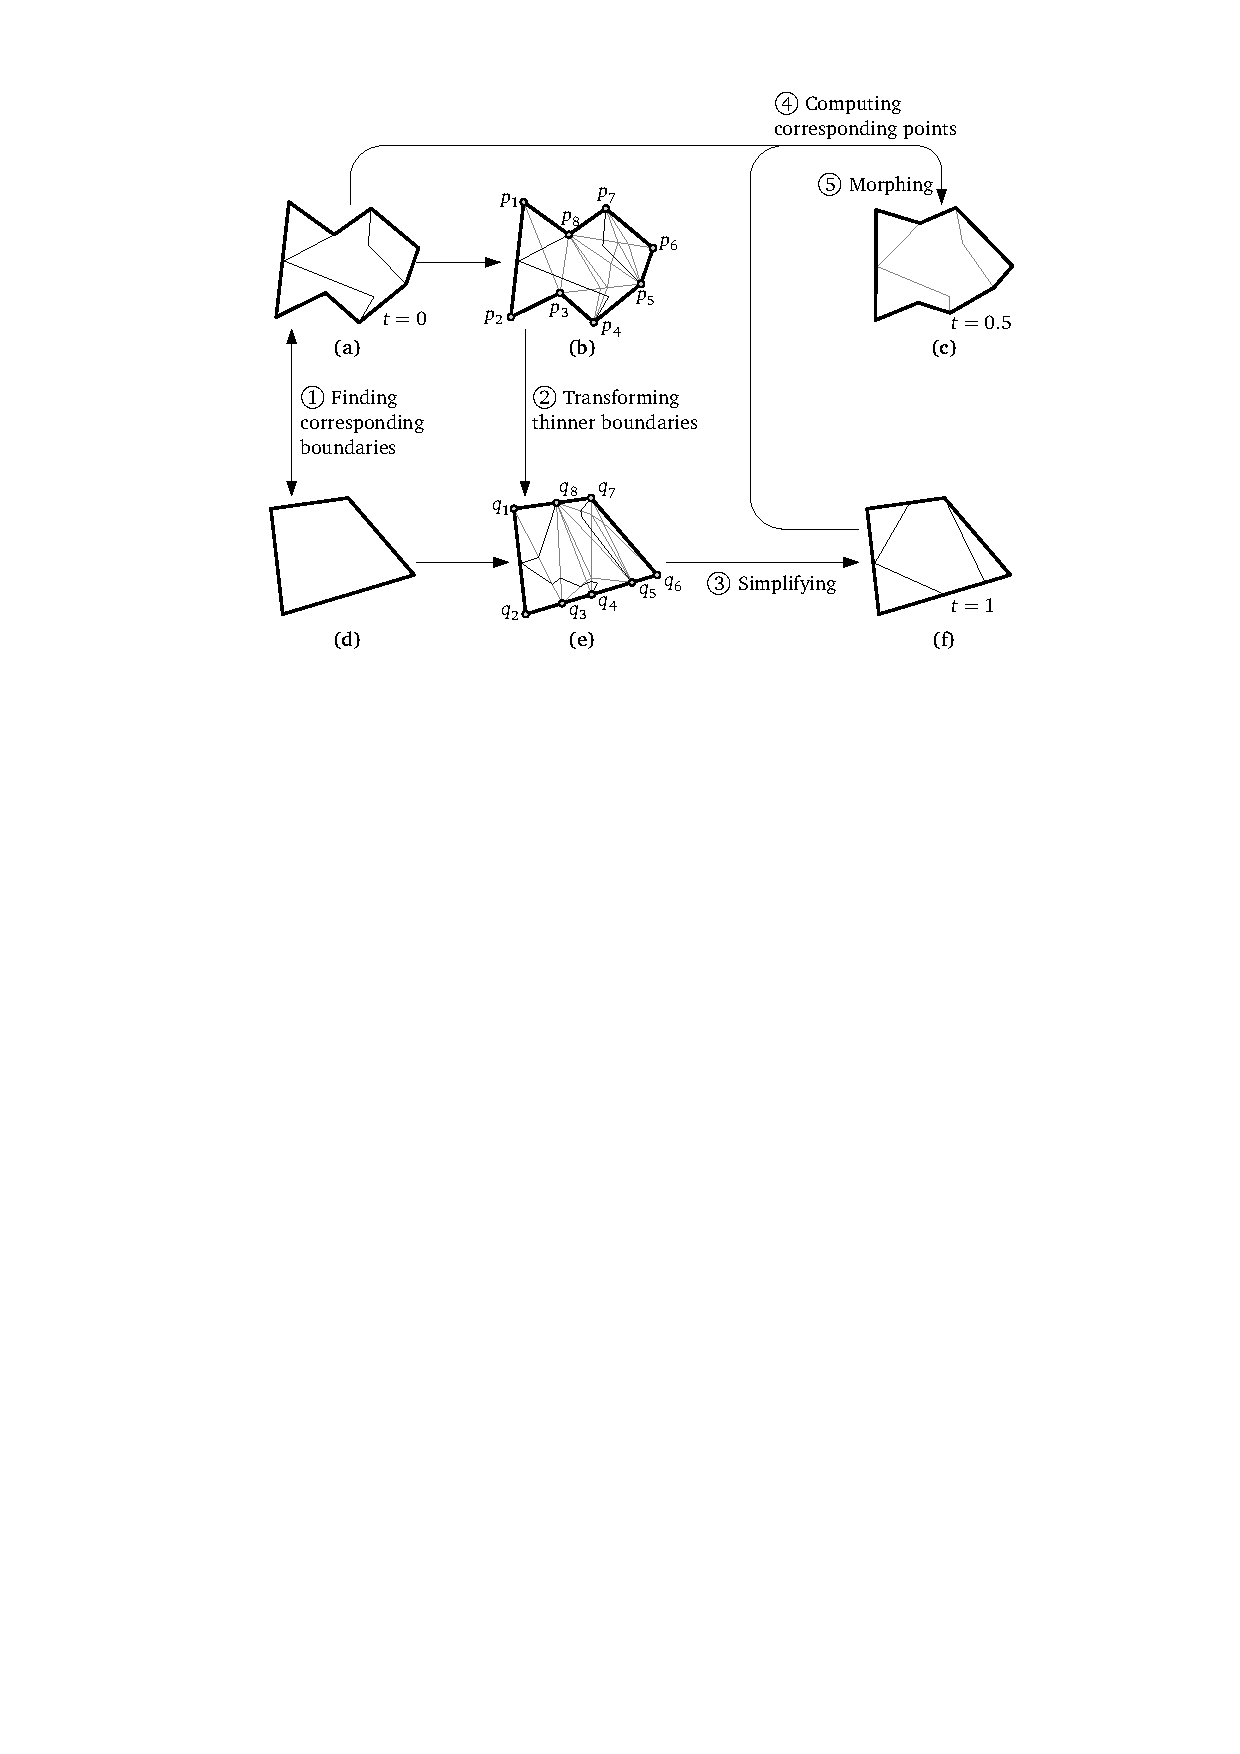
\includegraphics[page=1]{Admin_Introduction}
\caption{Framework of our method.
	The circled numbers indicate the steps. 
	(a)~The larger-scale administrative boundaries of a 
	region. 
	(d)~The smaller-scale administrative boundaries of the 
	same region as in~(a). 
	(b)~\&~(e) Constructing compatible triangulations for
	thicker polygons in~(a) and~(d) in order to 
	transform thinner boundaries in~(a) to~(e).
	(f)~The thinner boundaries are simplified from the 
	ones in~(e). 
	(c)~The result of continuous generalization
	by morphing when~$t=0.5$.
	The thinner boundaries in~(c) are being faded out.
	}
\label{fig:Admin_Introduction}
\end{figure}

Topological consistency is a property 
that must be attained in continuous generalization. 
In this chapter, we continuously generalize 
a two-level hierarchical subdivision---from 
a larger-scale map of administrative boundaries 
to a smaller-scale one.  
Our aim is to generate maps at any intermediate scales
without introducing topological conflicts.
For example, we try to generalize from
\fig\ref{fig:Admin_Introduction}a to
\fig\ref{fig:Admin_Introduction}d.
Our method consists of the following five steps.  

In step~\circled{1}, we find corresponding boundaries
between the two maps,
which are the thicker polylines in
\figs\ref{fig:Admin_Introduction}a 
and~\ref{fig:Admin_Introduction}d.  
We call the remaining boundaries, on the larger-scale map, 
\emph{unmatched} boundaries (see the
thinner polylines in \fig\ref{fig:Admin_Introduction}a). 
In order to achieve continuous generalization, 
we \emph{morph} (that is, deform continuously) 
between the thicker corresponding boundaries 
(see for example \textcite{Noellenburg2008}).
The unmatched boundaries must be morphed in a way 
that is consistent with the thicker corresponding boundaries.  
As there is no correspondence for the unmatched ones, 
we generate the corresponding boundaries 
in steps~\circled{2} and~\circled{3}.

In step~\circled{2}, we transform the thinner boundaries 
based on \emph{compatible triangulations} (CTs); 
see \figs\ref{fig:Admin_Introduction}b 
and~\ref{fig:Admin_Introduction}e. 
Two triangulations are \emph{compatible} 
if they have a correspondence of their vertex sets as well as 
the two triangulations are topologically 
equivalent~\parencite{Surazhsky2001}. 
With CTs, 
we can transform a thinner boundary in one triangulation 
(see \fig\ref{fig:Admin_Introduction}b) 
to a boundary in the other triangulation 
by traversing the triangles correspondingly 
(see \fig\ref{fig:Admin_Introduction}e). 
Therefore, if there is no conflict in one triangulation, 
then there is no conflict in the other triangulation.
 

In step~\circled{3}, we simplify the thinner boundaries using
the Douglas--Peucker algorithm~\parencite{Douglas1973} 
so that the thinner boundaries 
have the same complexities as the thicker ones 
(see \fig\ref{fig:Admin_Introduction}f). 
We use the simplified boundaries as the correspondences for 
the thinner boundaries in \fig\ref{fig:Admin_Introduction}a. 
On this basis, we are able to morph between
each pair (both thicker pairs and thinner pairs) of 
corresponding boundaries.
Since the thinner boundaries should not stay
on the smaller-scale map, 
we fade them out during morphing. 

We compute corresponding points 
for each pair of corresponding boundaries in step~\circled{4},
then we morph by interpolating between corresponding points 
in step~\circled{5}.

In order to achieve a topologically consistent workflow, 
we need to make sure that any of
steps~\circled{2}, \circled{3}, or~\circled{5}
must not introduce conflict.
In this chapter, we concentrate on accomplishing 
step~\circled{2}, the transformation step, 
without introducing topological conflicts.  
The topological consistency of the other two steps 
can be attained by employing the methods as proposed by
\textcite{Saalfeld1999} for step~\circled{3} and 
\textcite{GotsmanS2001} for step~\circled{5}.

For step~\circled{2},
we tested the rubber-sheeting method of \textcite{Doytsher2001} 
(making all vertices ``influential'').  
We soon noticed that resulting boundaries from that method 
often cross boundaries of the smaller-scale map. 
\fig\ref{fig:Admin_Rubbersheeting} shows such an example, 
which corresponds to \fig\ref{fig:Admin_Introduction}e. 
Similar problems occurred 
when we applied other variants of rubber-sheeting
(such as the one by \textcite{Haunert2005Conflation}).
That is why we decided to search for a more robust method.  
It turned out that 
CTs~\parencite{AronovSS93} can 
transform without introducing topological conflicts.  
The (quite old) idea is as follows.  
Suppose that point~$r_i$ is inside triangle~$\triangle{p_1p_2p_3}$. 
Then, this point can be expressed as a
\emph{unique} convex combination of 
\emph{simplicial coordinates}~$\lambda_{i,1}$, 
$\lambda_{i,2}$, and~$\lambda_{i,3}$ 
\parencite{Saalfeld1985-RS}:
\[
r_i=\lambda_{i,1}p_1+\lambda_{i,2}p_2+\lambda_{i,3}p_3,
\]
where $\lambda_{i,1}$, $\lambda_{i,2}$, $\lambda_{i,3}>0$, and
$\lambda_{i,1}+\lambda_{i,2}+\lambda_{i,3}=1$. 
We can \emph{uniquely} locate~$r_i$'s corresponding point~$s_i$ 
in a different triangle, say, $\triangle{q_1q_2q_3}$ 
by using the simplicial coordinates:
\[
s_i=\lambda_{i,1}q_1+\lambda_{i,2}q_2+\lambda_{i,3}q_3.
\]
Moreover, if two distinct points~$r_i$ and~$r_j$ are in the
same triangle, 
then we are able to locate their 
corresponding points~$s_i$ and~$s_j$ in another triangle 
such that~$s_i$ and~$s_j$ do not coincide.
If points~$r_i$ and~$r_j$ are in two different
triangles of a triangulation, 
then~$s_i$ and~$s_j$ can be located correspondingly 
in two triangles of the compatible triangulation. 
As a result, once we have CTs of two 
polygons, we can transform polylines consistently
(see \figs\ref{fig:Admin_Introduction}b 
and~\ref{fig:Admin_Introduction}e). 
CTs have been constructed by hand in order to compare
maps from different time periods \textcite{Fuse2004}. 
By contrast, we construct CTs
automatically, using the algorithm of \textcite{AronovSS93}.

%In the step of simplification, namely step of
%\fig\ref{fig:Admin_Introduction}(e) to~(f), we currently use 
%the 
%Douglas--Peucker
%algorithm in our implementation. In theory, this algorithm is not
%topologically consistent, that is, it may produce topological conflicts
%between the simplified boundaries and smaller-scale boundaries. We
%could easily replace the Douglas--Peucker algorithm, however, with an existing
%topologically consistent algorithm for line simplification, e.g., the
%algorithm of \citet{Saalfeld1999}. In the step of morphing (from
%\fig1(c) to~(f)), we simply use the straight-line trajectories 
%to
%interpolate. Also, this method is not topologically consistent in theory. We
%are planning to replace this algorithm with the topologically consistent
%morphing algorithm by \citet{Surazhsky2001}, which, as our method for
%the transformation step, is based on a CTs. 

Our contributions are as follows.
In \sect\ref{sec:Admin_OverallAlgorithm},
we propose a workflow based on CTs 
for generalizing administrative boundaries 
in a continuous and topologically consistent way. 
% To that end, we modify an existing dynamic programming algorithm for
% determining corresponding points to prepare for the construction of
% CTs.  and we show the details of computing the cost for 
%the dynamic
% programming algorithm; see Section~\ref{sec:Admin_MorphCorr}.  
%In
% Section~\ref{sec:Admin_MorphSinglePolylines}, and we show how 
%to morph
% single polylines using CTs to transform interior 
%polylines according
% to the differences of the boundaries.
We do a thorough case study for the boundaries of 
the counties and that of the provinces of Mainland China;  
We analyze the effectiveness and the efficiency of
our method in \sect\ref{sec:Admin_CaseStudy}.  
We conclude this chapter in \sect\ref{sec:Admin_Conclusions}.

\begin{figure}[tb]
	\centering
	\includegraphics[page=2]{Admin_Introduction}
	\caption{Crossings caused by the rubber-sheeting method of 
	\textcite{Doytsher2001}.}
	\label{fig:Admin_Rubbersheeting}
\end{figure}

\section{Methodology}
\label{sec:Admin_OverallAlgorithm}

Suppose that we have two maps  
of administrative boundaries:~\ml and~\ms.
The two maps represent the same area 
respectively at a larger scale and a smaller scale. 
We use a parameter~$t\in[0,1]$ 
to define the process of continuous generalization.
We continuously generalize from~\ml to~\ms
when~$t$ increases from~$0$ to~$1$.


As map~\ml is more detailed than map~\ms, 
a region of~\ms consists of several regions of~\ml. 
Consequently, a boundary on~\ms certainly 
has a corresponding boundary on~\ml, 
but a boundary on~\ml may not
have a correspondence on the smaller-scale map. 
We first find the \emph{corresponding boundaries} on the two maps.
We call the leftovers, on~\ml, the \emph{unmatched boundaries}. 
For a pair of corresponding boundaries, we
use a dynamic programming algorithm similar to the algorithm 
\textsc{Optcor}~\parencite{Noellenburg2008} to determine 
corresponding points.
Then, we morph between corresponding boundaries 
by using straight-line trajectories. 
For an unmatched boundary, we generate its correspondence on~\ms.
We transform the unmatched boundary based on compatible triangulations 
and then simplify the new boundary using the 
Douglas--Peucker algorithm~\parencite{Douglas1973}.
The boundary obtained from the simplification is used as 
the correspondence for the unmatched boundary.
As a result, we are able to morph 
between the unmatched boundaries and the generated ones. 
We fade out the morphing results of the unmatched boundaries
so that they will disappear when time~$t=1$.

The administrative regions are represented as polygons. 
An administrative region usually shares its boundary 
with some other administrative regions. 
These shared parts should be 
always shared even during the morphing.
Furthermore, we want to avoid processing a shared boundary twice.
For these reasons, we sometimes work on administrative boundaries
as a set of consecutive polylines instead of polygons.



\subsection{Finding corresponding polylines}
\label{sec:Admin_Preprocessing}

We match to find corresponding polylines 
from map~\ml and map~\ms.
The basic idea of our matching is the same as the polygon-based 
approach of \parencite{Fan2016Matching}, where they matched road 
networks based on urban blocks.
Given polygons on map~\ml and map~\ms, 
we find corresponding polylines using three steps. 
Note that if the inputs are boundaries of the polygons, 
i.e., polylines, 
we can easily generate the polygons 
based on \emph{doubly-connected edge list} 
\parencite[\chap2]{deBerg2008}.

First, we copy the polygons on~\ml and 
merge the copied polygons according to the polygons on~\ms. 
For each copied polygon, 
we try intersecting it with each polygon on~\ms and 
record the one that has the largest intersection area. 
Then, we merge all the copied 
polygons that record the same polygon on~\ms.

Second, we obtain matched polylines 
(i.e., corresponding polylines)
respectively from the boundaries of the 
merged polygons and the polygons on~\ms. 
We define that a vertex is an \emph{intersection node} 
if the vertex has degree at least 3. 
As the merged polygons and the polygons on~\ms 
have corresponding intersection nodes, 
we utilize these 
nodes to find corresponding polylines. 
We split the boundaries of the 
polygons at every intersection node, 
respectively for the merged polygons and the 
polygons on~\ms. 
(Note that two polygons on the same map may 
share some parts of their boundaries, 
it is sufficient to take only one copy of the shared parts.) 
Then we match the split boundaries of~\ml and~\ms  to get 
corresponding polylines. 
We use \emph{thicker} marks to 
present these corresponding polylines 
(see \figs\ref{fig:Admin_Introduction}a
and~\ref{fig:Admin_Introduction}d). 
Although there is a data-matching 
system~\parencite{Mustiere2008} 
available, we use a simple method to attain the matching. 
We match the split boundaries 
according to their intersection areas. 
The buffer-based method works well in our case study as 
corresponding polylines have relatively close positions.

Third, we extract unmatched polylines on~\ml. 
We split the boundaries of the polygons 
on~\ml at every intersection node, 
then we exclude all the split boundaries 
that overlay with the matched ones on~\ml. 
The remained polylines are the unmatched polylines on~\ml,
for which we use \emph{thinner} marks
(see \fig\ref{fig:Admin_Introduction}a). 

After the preprocessing, we have three types of polylines. 
The first one consists of 
the thicker (matched) polylines on~\ml
(see \fig\ref{fig:Admin_Introduction}a).
Each of them has a corresponding polyline on~\ms.
%
The second type consists of 
the thinner (unmatched) polylines on~\ml
(see \fig\ref{fig:Admin_Introduction}a).
each of which does not have a
corresponding polyline on~\ms.
%
The third type consists of 
the thicker (matched) polylines on~\ms
(see \fig\ref{fig:Admin_Introduction}d).

%We store the LSPs and the SSPs so that we know their correspondences whenever 
%we access them.

%
%detect three types of topological conflicts for the maps, i.e., 
%\emph{crossings}, \emph{unlinked ends}, and \emph{overlaps}. 
%%In our case studies, however, only crossings and unlinked ends occur; see 
%%\fig\ref{fig:Admin_Preprocessing}(a). 
%Instead of detecting the three topological conflicts for polylines, we test 
%the relationships of any pair of edges, which is easier to implement but still 
%discovers all the conflicts. The relationship of a pair of edges can be 
%\emph{disjoint}, \emph{touch}, \emph{link}, \emph{crossing}, or 
%\emph{overlap}, 
%where \emph{link} means that two edges share an end and \emph{touch} means one 
%end of an edge is on another edge. If two edges link each other, then the 
%shared end vertex has degree at least two. We identify unlinked ends by 
%counting degrees of the two end vertices of each edge. If a vertex has degree 
%one, then this vertex is an unlinked end. To make this detection more 
%efficient, we use a grid-based algorithm similar to that mentioned by 
%\cite{pw-wyds-GISRUK14} instead of a brute-force search. We detect these 
%topological conflicts automatically, and correct them manually; see 
%\fig\ref{fig:Admin_Preprocessing}(a).
%
%\begin{figure*}[htb]
%  \centering
%  \includegraphics{Admin_figures/Preprocessing.eps}
%  \caption{Preprocessing for a map.}
%  \label{fig:Admin_Preprocessing}
%\end{figure*}
%
%Second, we split polylines at each intersection, where an intersection is a 
%vertex of degree at least 3. As shown in 
%\fig\ref{fig:Admin_Preprocessing}(b), 
%the line segment to the right side of the intersection was a part of the red 
%polyline on the larger-scale map, while a part of the thinner 
%polyline on the 
%smaller-scale map. Thus it was difficult to determine correspondence relations 
%between these polylines. By contrary, we can easily find the three pairs of 
%corresponding polylines after splitting the original polylines at 
%intersections 
%(see the polylines in the right side of~\ref{fig:Admin_Preprocessing}(b)).
%
%Third, we unite two polylines that \emph{touch} each other if the degree of 
%the \emph{touch vertex} is exactly 2. This is also useful for finding 
%corresponding polylines; see 
%\fig\ref{fig:Admin_Preprocessing}(c). Up to now, 
%we are sure of two aspects. One aspect is that a polyline always connects two 
%intersections, that is, there is no touch vertex with degree 2 anymore. The 
%other aspect is that an intersection is always an end vertex of a polyline. 
%This means a polyline will never go through an intersection. We do the second 
%and third preprocessing steps by constructing a doubly-connected edge list 
%\cite{Berg2008}, and then traversing along edges to extract polylines.
%
%Fourth, we match polylines from the two maps, and unite larger-scale polylines 
%according to smaller-scale polylines; see 
%\fig\ref{fig:Admin_Preprocessing}(d). Usually, there are 
%several larger-scale 
%polylines corresponding to one smaller-scale polyline. We unite these 
%larger-scale polylines and take the result as the correspondence of a 
%smaller-scale one. To match polylines, we construct their buffers with a 
%radius 
%$r$, where we set $r$ to the middle value of the edge lengths of the 
%larger-scale polylines. For the buffer of a larger-scale polyline, we overlap 
%it with the buffer of a smaller-scale polyline. If the overlap area is larger 
%than a threshold, then this larger-scale polyline probably corresponds to the 
%smaller-scale polyline. We say that they are candidates for each other. 
%Usually, a larger-scale polyline has one candidate, and a smaller-scale 
%polyline has more than one candidate. We unite a smaller-scale polyline's 
%candidates to create a new polyline. This new polyline is the corresponding 
%polyline of the smaller-scale one. An exception is that a very short 
%larger-scale polyline may have more than one candidate. In this case, we 
%report 
%it and manually unite the polylines.

%The following paragraph might have been 
%presented******************************************************************
%Now we have three sets of polylines. The first one is the set of larger-scale 
%polylines (LSPs) each of which has a smaller-scale corresponding polyline; see 
%the thicker polylines in \fig\ref{fig:Admin_Introduction}(a). 
%The second one is 
%the set of larger-scale polylines which do not have a smaller-scale 
%corresponding polyline. We call them single polylines (SPs); 
%see the thinner 
%polylines in \fig\ref{fig:Admin_Introduction}(b). The third set 
%contains the 
%smaller-scale polylines (SSPs); see the thicker polylines in 
%\fig\ref{fig:Admin_Introduction}(d). We store the LSPs and the 
%SSPs 
%correspondingly so that we are able to know the correspondences directly when 
%we access the data.

\subsection{Morphing a polyline to its corresponding polyline}
\label{sec:Admin_MorphCorr}

For a pair of corresponding polylines, 
one being a thicker polyline on~\ml and 
the other being a thicker polyline on~\ms, 
we use a variant of 
the dynamic programming algorithm \textsc{Optcor} 
of \textcite{Noellenburg2008} 
to compute corresponding points 
(possibly injecting additional
vertices).
%In stead of ultilizing the linear interpolation algorithm 
%(citation) to the pair of polylines, \textsc{Optcor} apply it 
%to the 
%pairs of subpolylines. The problem is to determine 
%corresponding 
%subpolylines. (improve this section accordingly)
The algorithm \textsc{Optcor} models the problem of 
computing corresponding points as 
finding an optimum correspondence, 
with respect to a cost function.
\textsc{Optcor} considers three cases of a 
correspondence for an edge, namely, 
the edge corresponds to a vertex, 
to an edge, or to a merged sequence of edges.
We call all the three cases corresponding subpolylines
as a point or an edge is a degenerate subpolyline. 

For a pair of corresponding subpolylines, 
\textcite{Noellenburg2008} define the cost 
as a combination of three values: 
(i)~the distance between the corresponding points, 
(ii)~the length difference of the pair of subpolylines, and 
(iii)~the changes of the vectors between corresponding points. 
Then \textsc{Optcor} computes corresponding points 
by ``looking back'' to combine 
the last $1,2,\ldots, or~k$ edges as a subpolyline, 
while minimizing the cost over 
the whole pair of corresponding polylines. 
Here, $k$ is a user-specified parameter, 
which gives a trade-off between quality and efficiency.

To make the problem simple, 
our variant considers only the first value in their cost, 
that is, the distance between corresponding points. 
We denote this distance by~$\delta$.  
In order to compute the cost function, we linearly
interpolate between each pair of corresponding subpolylines 
so that each vertex on one subpolyline has a, possibly injected, 
corresponding vertex on the other one.
The pairs of corresponding vertices
subdivide the (sub)polylines into corresponding line segments
(see \fig\ref{fig:Admin_BasicConcepts}).  
A line segment is (part of) an edge of a polyline. 
The cost of a pair of (whole) polylines is 
the sum of the costs for each pair of 
corresponding line segments. 
The cost for a pair of corresponding line segments 
is computed as follows.

\begin{figure}[tb]
	\centering
	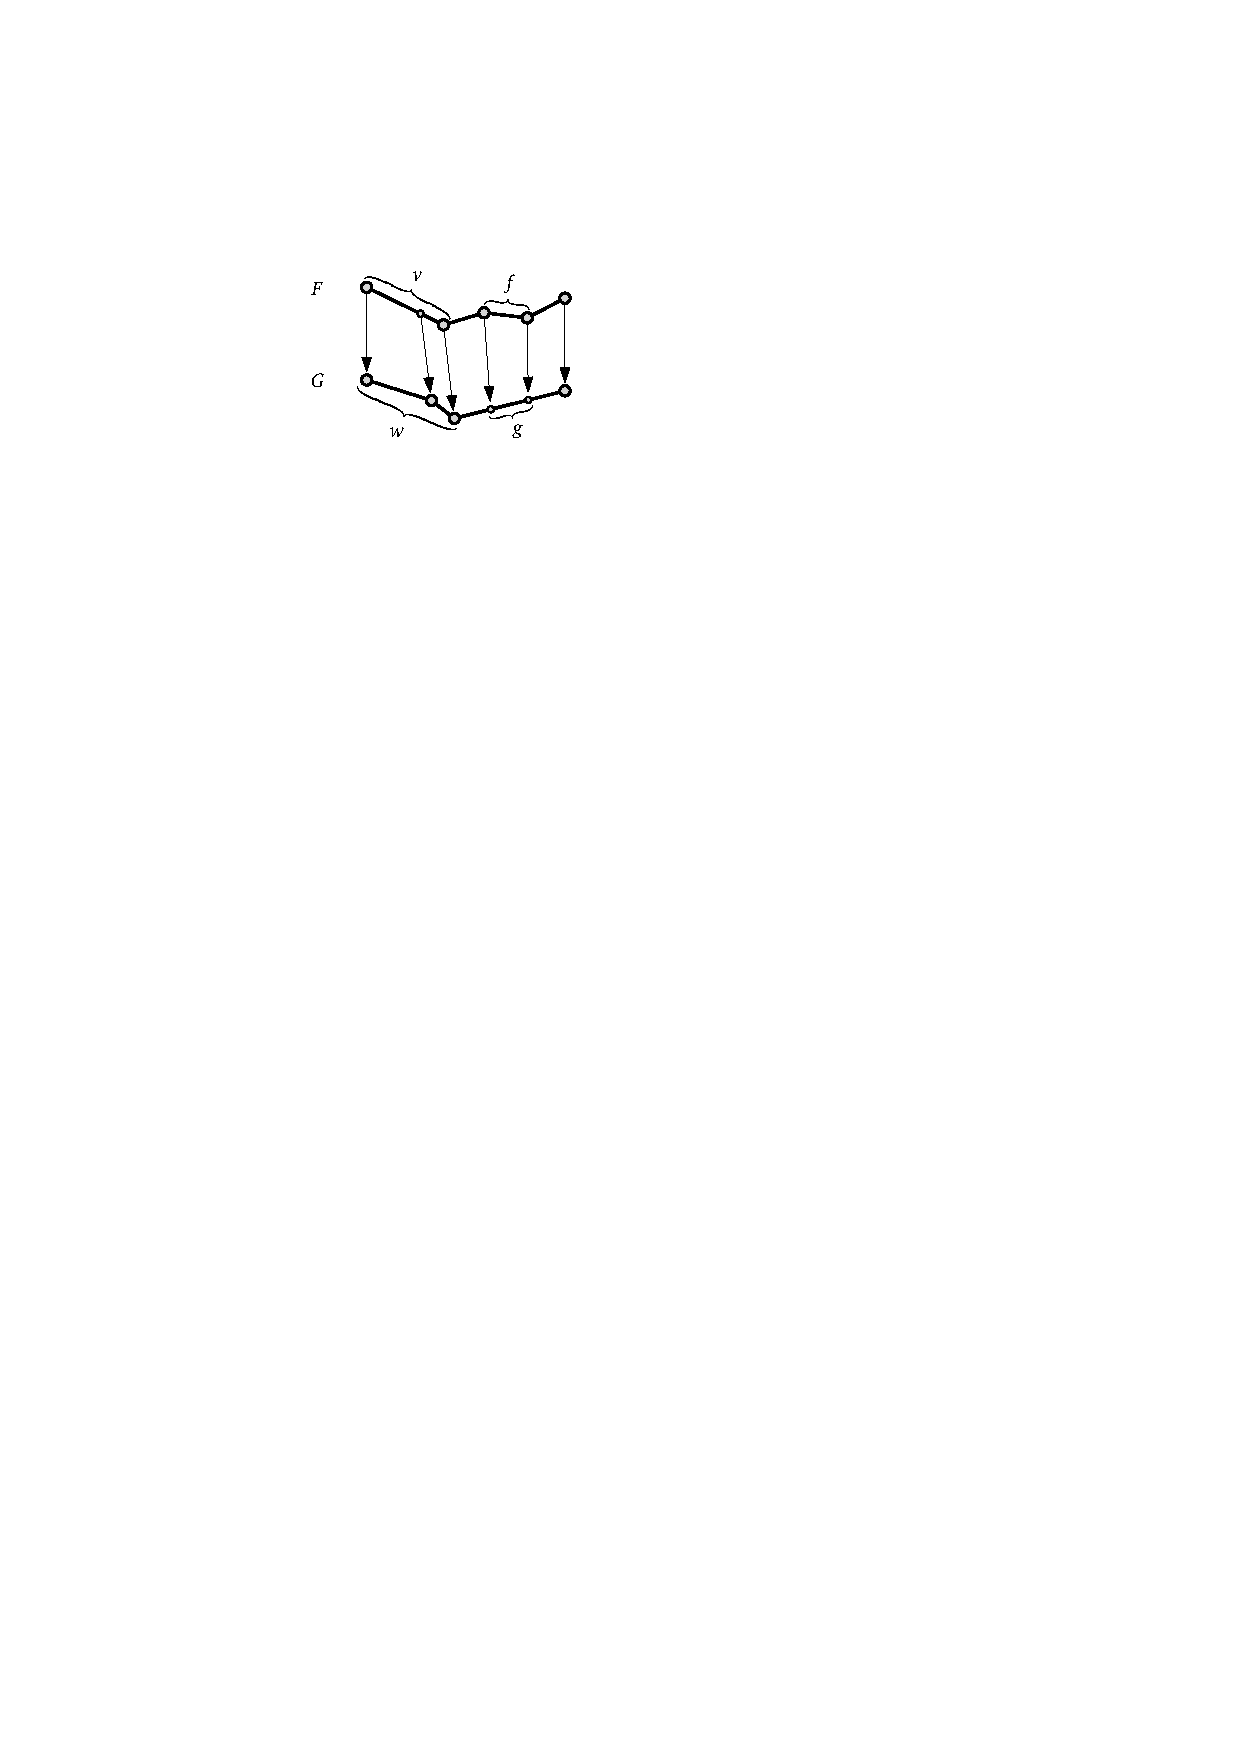
\includegraphics[page=1]{Admin_MorphCorr}
	\caption{Corresponding polylines:~$F$ and~$G$,
		corresponding subpolylines:~$v$ and~$w$,
		and corresponding line segments:~$f$ and~$g$.}
	\label{fig:Admin_BasicConcepts}
\end{figure}

Let polyline~$F$ on~\ml and polyline~$G$ on~\ms 
be a pair of corresponding polylines. 
Let~$f=\overline{\alpha(0)\alpha(1)}$ 
be a line segment on~$F$, and 
let~$g=\overline{\beta(0)\beta(1)}$ 
be a line segment on $G$ that corresponds to~$f$. 
Let~$\alpha(0)=(x_1,y_1)$, $\alpha(1)=(x_2,y_2)$, 
$\beta(0)=(x_3,y_3)$, and~$\beta(1)=(x_4,y_4)$, 
which are already known. 
The coordinates of a pair of 
corresponding points~$\alpha(u) \in f$ 
and~$\beta(u) \in g$ are
\begin{align}
	\alpha(u)=(1-u)\alpha(0) + u \alpha(1), \nonumber \\
	\beta(u)=(1-u)\beta(0) + u \beta(1). \nonumber 
\end{align}
When we morph~$f$ to~$g$, 
we move each point~$\alpha(u)$ 
to its corresponding point~$\beta(u)$;
see \fig\ref{fig:Admin_Integral_Correspondence}.
We define the cost of this morphing
as the integral over the distances between all the pairs of 
corresponding points, that is,
\[
\delta(f, g)=\int_{0}^{1}|\beta(u) - \alpha(u)|du,
\]
where~$|\beta(u) - \alpha(u)|$ is the Euclidean distance 
between~$\alpha(u)$ and~$\beta(u)$, 
which can be represented as~$\sqrt{au^2+bu+c}$. 
The coefficients~$a$, $b$, and~$c$ are dependent on 
the coordinates of~$\alpha(0)$, $\alpha(1)$, $\beta(0)$, 
and~$\beta(1)$, as follows. 
\begin{align}
	a=~&(x_1-x_2-x_3+x_4)^2+(y_1-y_2-y_3+y_4)^2,  \nonumber \\
	b=~&-2(x_1-x_3)(x_1-x_2-x_3+x_4) \nonumber \\
	   &-2(y_1-y_3)(y_1-y_2-y_3+y_4),  \nonumber \\
	c=~&(x_1-x_3)^2+(y_1-y_3)^2. \nonumber
\end{align}
Let~$X=au^2+bu+c$. 
We have~$a\geq0$ and, 
since~$X\geq0$ ($X$ is the square of a Euclidean distance), 
$\Delta=4ac-b^2\geq0$. 
Note that, if~$a=0$, then~$b=0$. Let
\[
\delta(f, g)=\int_{0}^{1}|\beta(u) - \alpha(u)|du=\int_{0}^{1}\sqrt{X}du.
\]
Then $\delta(f, g)$ can be computed, according to 
\textcite[p.~1064, 
integrals~241 and~245]{Bronstein2001}, as follows:
\[
\delta(f, g)=\\
\begin{cases}
\sqrt{c}u|_0^1 & \text{if } a=0,\\
\frac{(2au+b)\sqrt{X}}{4a}|_0^1 & \text{if } a>0, \Delta=0,\\
\frac{(2au+b)\sqrt{X}}{4a}|_0^1 + 
\\\frac{\Delta}{8a\sqrt{a}}\ln(2\sqrt{aX}+2au+b)|_0^1 & \text{if } a>0, 
\Delta>0.
\end{cases}
\]

\begin{figure}[tb]
\centering
\includegraphics[page=2]{Admin_MorphCorr}
\caption{Corresponding points of 
a pair of corresponding line segments.}
\label{fig:Admin_Integral_Correspondence}
\end{figure}

Cost~$\delta$ can be regarded as the average distance of 
moving each~$\alpha(u)$ to each~$\beta(u)$.
\fig\ref{fig:Admin_IntegralComputation} 
shows a few examples of computing~$\delta$. 
We obtain the optimum correspondence by
minimizing the cost of moving between corresponding points, 
where the lengths of line segments are used as weights:
\[
\delta(F,G) =
\min_
{\substack
	{\pi \text{: correspondence} \\ 
		\text{between $F$ and $G$}
	}
} 
\sum_
{\substack
	{f\in F \text{ and }g\in G, \\ 
		\text{ where } f \text{ corresponds to } g \text{ in } 
		\pi
	}
}
\frac{|f|+|g|}{2} \delta(f,g).
\]
In other words, there can be many choices of 
defining corresponding points
(see \fig\ref{fig:Admin_ChooseCorrespondence}),
but we choose the one that minimizes cost~$\delta(F,G)$.


\begin{figure}[tb]
\centering
\includegraphics[page=3]{Admin_MorphCorr}
\caption{Examples of computing $\delta(f,g)$. 
The values in the subfigures 
represent the lengths of the edges.}
\label{fig:Admin_IntegralComputation}
\end{figure}

\begin{figure}[tb]
\centering
\includegraphics[page=4]{Admin_MorphCorr}
\caption{Three possible ways of defining corresponding points
	between the two polylines.
	Correspondence $\pi_2$ is the one 
	that minimizes cost~$\delta(F,G)$.
}
\label{fig:Admin_ChooseCorrespondence}
\end{figure}

Recall that \textsc{Optcor} considers three cases of a 
correspondence for an edge. 
We find that the first case, an edge corresponding to a vertex, 
may result in different numbers of vertices 
on the two polylines.  
Our major modification is removing this case 
from the algorithm.
This change ensures that
a pair of corresponding polylines 
will eventually have the same 
numbers of vertices (or line segments).
This property is essential for 
constructing CTs, 
which are used later in our workflow.  
We name our modified version \textsc{Optcor-s}, 
where letter \emph{S} stands for \emph{Simplified}.

Suppose that there are originally~$n_F$ vertices on~$F$ 
and~$n_G$ vertices on~$G$,
\textsc{Optcor-s} requires that 
the look-back parameter~$k$ is bounded from below 
by~$n_F/n_G$ and~$n_G/n_F$. 
Otherwise, there will be at least one segment 
that corresponds to a vertex. 
In our experiments, we always use a (large) value of~$k$ 
that produces results with high quality 
(in the sense of the dynamic-programming algorithm). 
We morph by interpolating between corresponding points using
straight-line trajectories. 
\fig\ref{fig:Admin_MorphCorr} shows an example
with~$0.25$, $0.5$, and~$0.75$ for~$t$.

\begin{figure}[tb]
\centering
\includegraphics[page=5]{Admin_MorphCorr}
\caption{Morphing polyline $F$ to its corresponding 
    polyline $G$. 
    The arrows show the moving trajectories of the vertices.}
\label{fig:Admin_MorphCorr}
\end{figure}

Some other algorithms for computing corresponding points 
can be used (e.g., linear interpolation). 
We observed that an algorithm which
computes corresponding points more carefully 
can yield better results, 
meaning that the interpolated polylines 
are more similar to the two sources and
crossings are less likely introduced.
Some sophisticated algorithms can be 
considered to define the interpolation trajectories, 
such as geodesic shortest paths~\parencite{Bereg2005}, 
b-morphs~\parencite{Whited2011BallMorph}, 
or a method based on 
least squares adjustment~\parencite{Peng2013LSA}. 
Specifically, it is possible to use CTs
not only for the transformation step (as in our method) 
but also to ensure the topological consistency in the morphing step~\parencite{GotsmanS2001,Surazhsky2003Intrinsic,Surazhsky2004HighQuality}.

%title displays in contents
\subsection[Morphing a polyline to 
its generated corresponding polyline] 
{Morphing a polyline to 
its generated corresponding polyline \\ during fade-out}
\label{sec:Admin_MorphSinglePolylines}

For the thinner polylines on~\ml, 
morphing them must be consistent with 
what we do to the thicker corresponding polylines. 
To achieve this, we generate their corresponding polylines, that is, thinner polylines on~\ms. 
We transform the thinner polylines on~\ml based on CTs
to get a set of new polylines.
Then, we simplify these new polylines 
to generate the thinner polylines on~\ms,
where we use the Douglas--Peucker algorithm
\parencite{Douglas1973}.

We construct a pair of CTs
for each pair of polygons correspondingly bounded
by the thicker polylines on~\ml and 
the thicker polylines on~\ms
(see \figs\ref{fig:Admin_Introduction}b
and~\ref{fig:Admin_Introduction}e). 
We call them the \emph{triangulation on~\ml} and 
the \emph{triangulation on~\ms}. 
Constructing CTs requires that
the two polygons have the same number of vertices,
which have been attained by using \textsc{Optcor-s}
(see \sect\ref{sec:Admin_MorphCorr}). 
We use the algorithm of \textcite{AronovSS93}
to construct CTs. 
For the two polygons both with $m$ vertices, 
we triangulate them independently
(see \figs\ref{fig:Admin_ConstructCTs}a 
and~\ref{fig:Admin_ConstructCTs}b). 
Then we create a regular~$m$-gon and 
map the chords of the two triangulations 
into the regular~$m$-gon
(see \figs\ref{fig:Admin_ConstructCTs}c). 
The mapped chords may cross with each other.
We use the crossings as dummy vertices and
split the mapped chords
(see \figs\ref{fig:Admin_ConstructCTs}d). 
As a matter of fact, these dummy vertices are called 
\emph{steiner points} \parencite{AronovSS93}.
These split chords may produce some convex faces
(see \fig\ref{fig:Admin_ConstructCTs}d).
We triangulate each convex face
that has more than three vertices. 
To triangulate, we select one vertex and 
add edges between 
this vertex to each of the other vertices, 
except the two immediate-neighboring ones. 
After triangulating, we have 
a \emph{combined} triangulation
(see \fig\ref{fig:Admin_ConstructCTs}e).
We map the combined triangulation 
(including steiner points and new edges)
back to modify the two original triangulations. 
By the modification, we have a pair of 
CTs of the two original polygons
(see \figs\ref{fig:Admin_ConstructCTs}f 
and~\ref{fig:Admin_ConstructCTs}g).

\begin{figure}[tb]
\centering
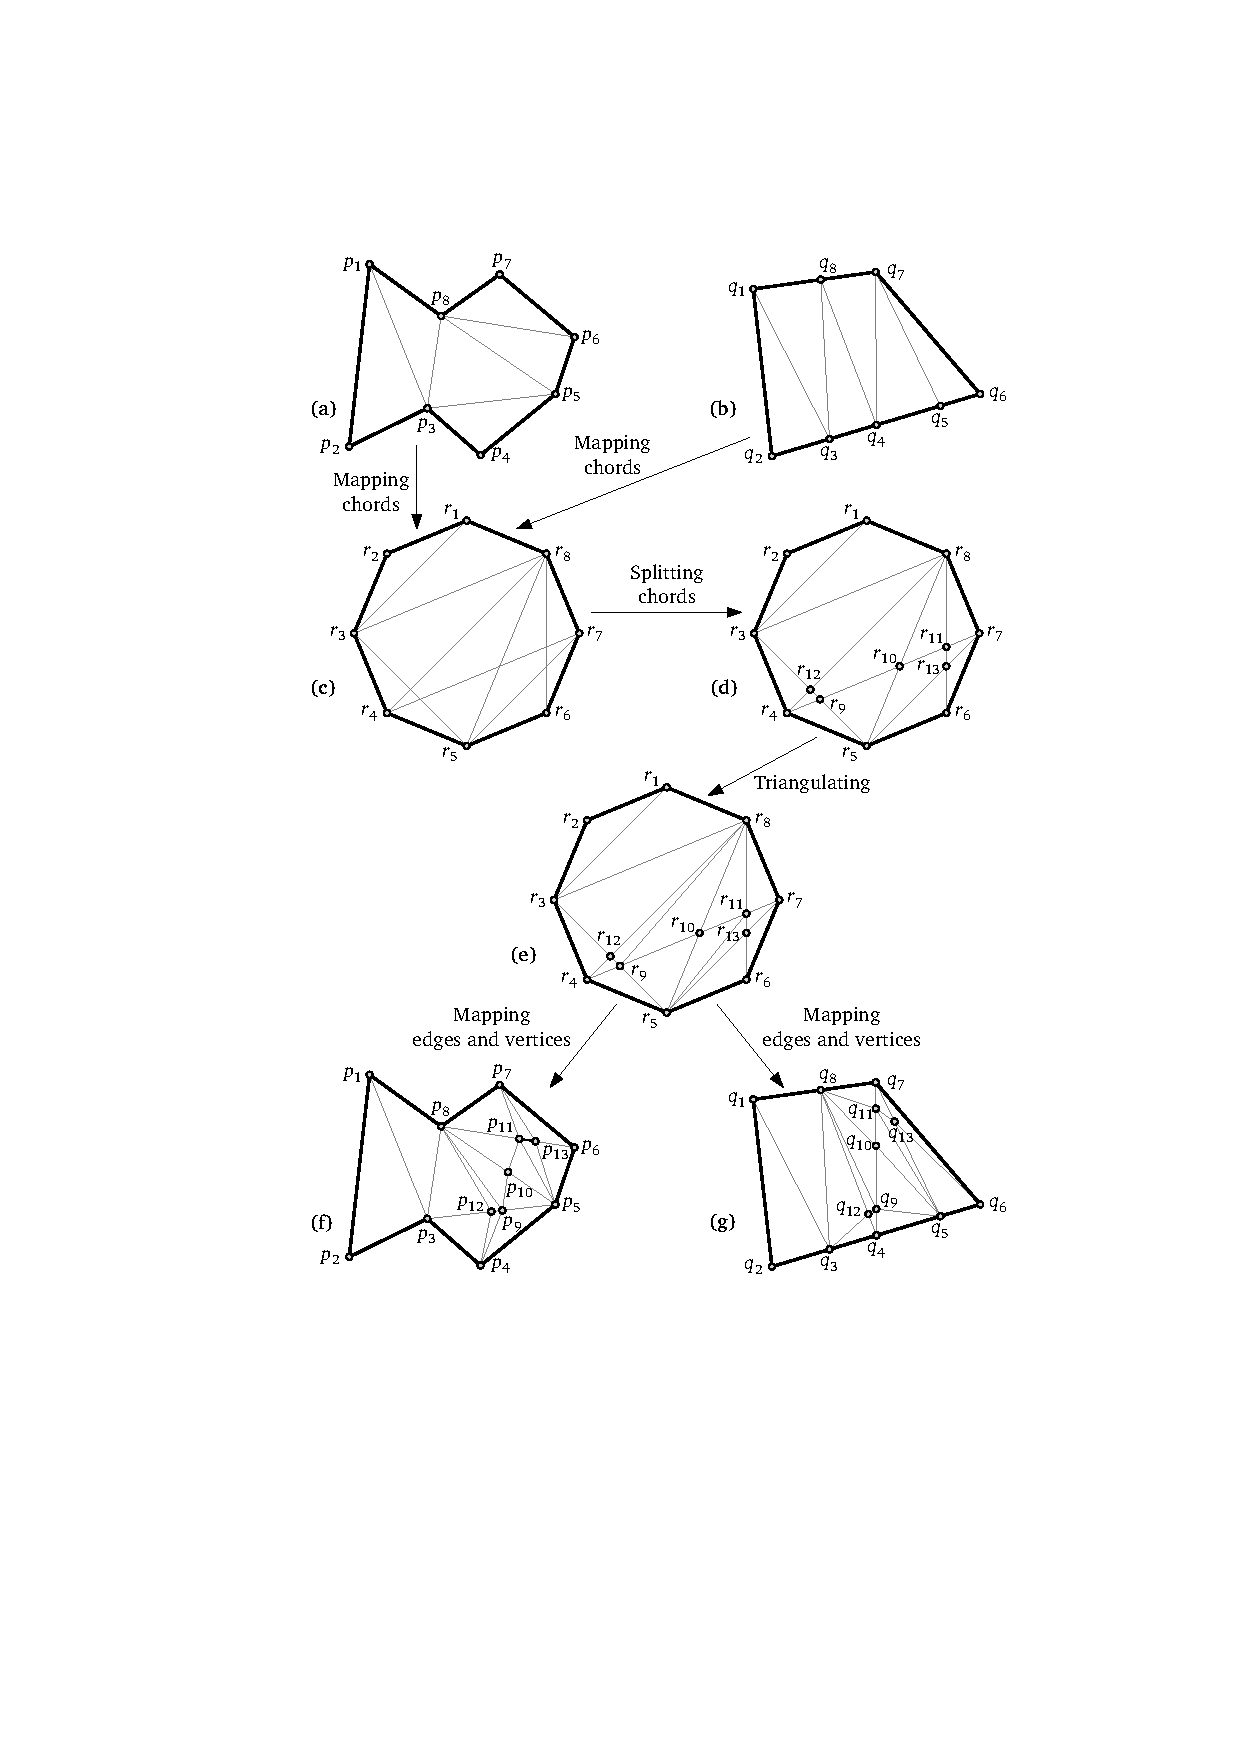
\includegraphics[page=1]{Admin_MorphSingle}
\caption{Constructing compatible triangulations.}
\label{fig:Admin_ConstructCTs}
\end{figure}


With the CTs, 
we transform the thinner polylines in the 
triangulation on~\ml to the polylines on~\ms, 
according to simplicial coordinates. 
The new polylines should traverse exactly the ``same'' 
triangles as thinner polylines on~\ml.
To this end, we compute the crossings 
between thinner polylines and 
the edges of the triangulation; 
then, we also transform these crossings
into the triangulation on~\ms. 
Because of the crossings, the new polylines have
more vertices than the thicker polylines on~\ml. 
While our aim is to generate polylines that have
the same density of vertices as the thicker polylines on~\ms. 
Hence, we simplify the new polylines 
(see \fig\ref{fig:Admin_Introduction}f). 
For a \emph{thinner hole} (polygon) on~\ms, 
we keep at least three vertices during simplification 
to avoid degenerating
it to a straight line or a point.
We call the simplified polylines 
the \emph{thinner polylines on~\ms}.

Again, we use algorithm \textsc{Optcor-s} 
to compute corresponding points
for each pair of corresponding thinner polylines, 
which are respectively on~\ml and~\ms. 
We use straight-line trajectories
to interpolate between corresponding points. 
As the thinner polylines do not exist when~$t=1$, 
we fade them out during the morphing process. 
An example is shown in \fig\ref{fig:Admin_Introduction}c.

\subsection{Running time}
\label{sec:Admin_Runningtime} 

We analyze the running time for a pair of polygons correspondingly bounded by 
the thicker polylines on~\ml and the thicker polylines on~\ms. 
We use $N$ to denote 
the number of vertices of the polygon on~\ml, 
$n$ the number of vertices of the polygon on~\ms, 
and $N'$ the number of vertices of all the thinner polylines 
inside the polygon on~\ml. 
For simplicity, we assume that $O(N')\in O(N)$.

Constructing the CTs takes time~$O(N\log N + l)$ 
according to \textcite{AronovSS93}, 
where~$O(l)\in O(N^2)$ is the number of steiner points 
inserted during the construction.
Simplifying the polylines resulted from transformation, 
using the Douglas--Peucker algorithm, 
costs time 
$O(N(N+l)\log{N})$~\parencite{Hershberger92speedingup}.  
\textsc{Optcor-s} takes time~$O(k^2Nn)$ 
to compute corresponding points, 
where~$k$ is the look-back parameter. 
Fortunately, outputting the representation at a target scale 
only takes time~$O(N)$.
Therefore, our method is feasible in real time. 
In fact, for each (possibly injected) vertex~$p$ on~$F$ 
we store a representation such as~$p(t)=(1-t)p+tq$,
where~$q$ is the vertex on~$G$ that corresponds to~$p$. 
In our implementation, computing corresponding points
is the by far most time-consuming step.



\section{Case Study}
\label{sec:Admin_CaseStudy}

We implemented our method based on 
C\# (Microsoft Visual Studio~2010) and ArcGIS Engine~10.1. 
We ran our case study under 
Windows~7 on a $3.3\,$GHz dual core CPU with $8\,$GB RAM. 
We measured time consumption based on the
built-in C\# method System.Environment.TickCount.

We tested our method 
on the administrative boundaries of Mainland China
(see \figs\ref{fig:Admin_Data}a and~\ref{fig:Admin_Data}c),
which are from 
the National Fundamental Geographic Information System 
and are based on the projected coordinate system 
\emph{Krasovsky 1940 Lambert Conformal Conic}. 
We removed the enclave in Gansu province 
as well as all the islands.
%
We used county boundaries (see \fig\ref{fig:Admin_Data}a)
and provincial boundaries (see \fig\ref{fig:Admin_Data}c),
where the polylines have been preprocessed
(see \sect\ref{sec:Admin_Preprocessing}).
%
Since we can hardly see the details
if we present the whole map, 
we focus on a small portion, say, 
Tianjin province\footnote{Interactive animations 
of more	provinces are available at
\url{http://www1.pub.informatik.uni-wuerzburg.de/pub/data/agile2016/}.
(We recommend opening the website with Google Chrome.)}
(also known as Tianjin municipality);
see \figs\ref{fig:Admin_Data}b and~\ref{fig:Admin_Data}d.

\begin{figure}[tb]
\centering
\includegraphics{Admin_CaseStudy_Data}
\caption{Administrative boundaries of Mainland China.}
\label{fig:Admin_Data}
\end{figure}

\fig\ref{fig:Admin_CaseStudy} shows our results of Tianjin.
Recall that our aim is to continuously generalize 
from counties~\ml to provinces~\ms. 
According to the provincial boundaries in
\fig\ref{fig:Admin_CaseStudy}c, we are able to
distinguish the hierarchies of the county boundaries in
\fig\ref{fig:Admin_CaseStudy}a 
Then, we find the matched polylines 
(the thicker ones in \figs\ref{fig:Admin_CaseStudy}a 
and~\ref{fig:Admin_CaseStudy}c) and the unmatched polylines 
(the thinner ones in\fig\ref{fig:Admin_CaseStudy}a); see 
step~\circled{1}.

\begin{figure}[tb] 
\centering
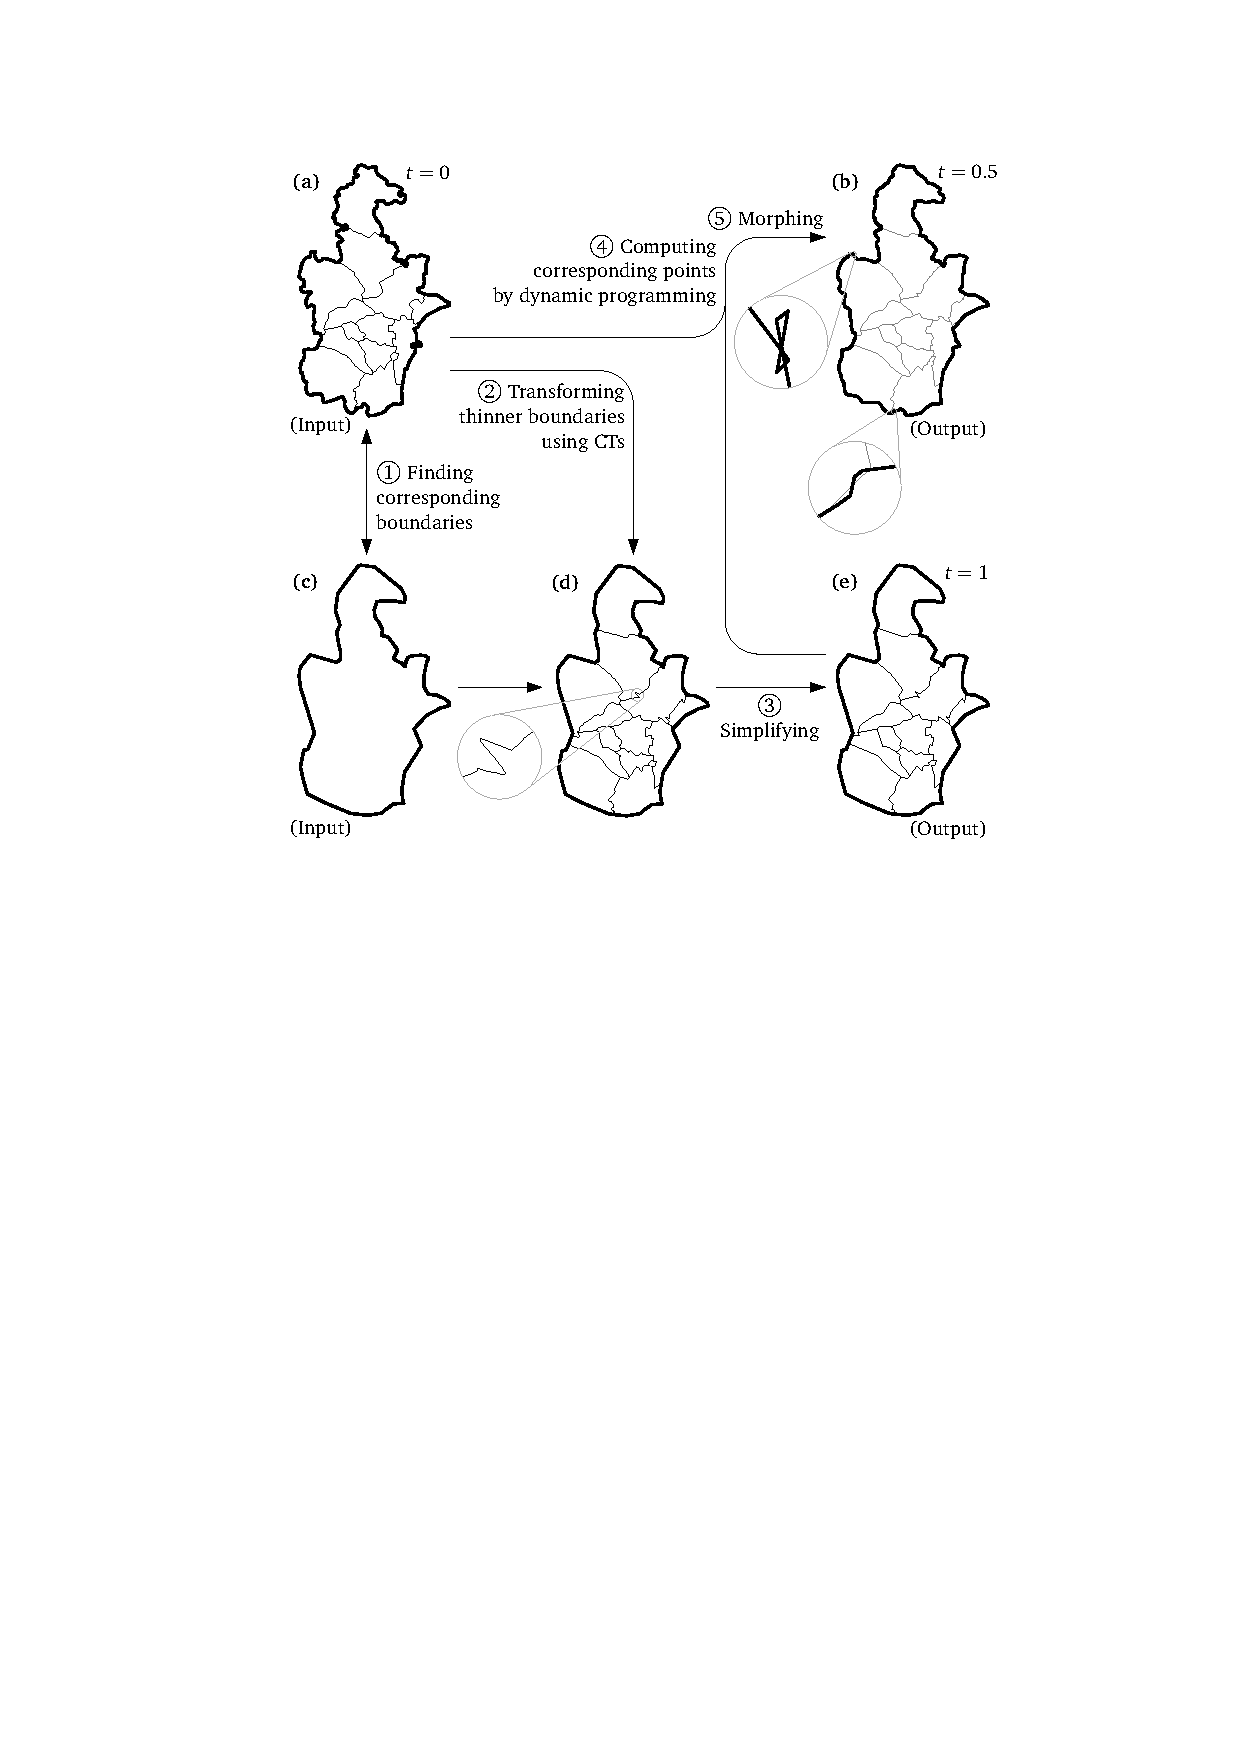
\includegraphics[page=1]{Admin_CaseStudy_Results}
\caption{Case study on administrative boundaries
    of Tianjin province.
	The circled numbers indicate the step orders, 
	analogous to \fig\ref{fig:Admin_Introduction}.     
	For the sake of legibility, 
    we did not display the CTs. 
	Continuous generalization is achieved by 
	morphing from~(a) to~(e).  
	The thinner boundaries in~(b) are being faded out
	during the morphing.}
\label{fig:Admin_CaseStudy}
\end{figure}

In step~\circled{2}, we transform the thinner boundaries in 
\fig\ref{fig:Admin_CaseStudy}a
so that there are corresponding thinner boundaries on~\ms
(see \fig\ref{fig:Admin_CaseStudy}d).
Recall that we compute corresponding points between 
corresponding thicker polylines using \textsc{Optcor-s}
and then transform thinner polylines based on CTs.
When computing corresponding points, 
we used the fact that the~$90$ thicker polylines 
(with~$55{,}533$ vertices) on~\ml and 
the~$90$ thicker polylines (with~$7{,}527$ vertices) on~\ms 
shared many vertices (\ms may be generalized from~\ml).
We split the thicker polylines, on~\ml and~\ms, 
into many subpolylines according to the shared vertices. 
We computed corresponding points for each pair of subpolylines, 
which was much faster than computing without the splitting. 
Using look-back parameter~$145$, 
the computation takes time~$266\,$s 
with cost~$\sum \delta(F,G)=125{,}050\,\mathrm{km}^2$. 
Value~$145$ is the smallest look-back parameter
that achieves the optimum result in
the sense of the dynamic programming algorithm. 
Constructing the CTs costs $168\,$s. 
There is no conflict \mine{for the new polylines} in
\fig\ref{fig:Admin_CaseStudy}d. 
However, a flaw is that there are some zigzags 
caused by our transformation
(see for example the enlarged figure next to 
\fig\ref{fig:Admin_CaseStudy}d)
%
We also tested transforming by the rubber-sheeting method of 
\textcite{Doytsher2001}, 
which, unfortunately, introduced~$39$ crossings. 

In step~\circled{3}, we simplified the thinner polylines 
in \fig\ref{fig:Admin_CaseStudy}d
using the Douglas--Peucker algorithm. 
This simplification took $29\,$s 
and caused~$8$ crossings as well as~$2$ overlaps. 
We corrected the~$10$ conflicts by hand. 
Note that we can avoid these conflicts by using
a topologically consistent line simplification method, 
e.g., the algorithm of \textcite{Saalfeld1999}.

In step~\circled{4}, we use \mbox{\textsc{Optcor-s}} 
to compute corresponding points between 
the~$5{,}819$ thinner polylines 
(with~$438{,}092$ vertices) on~\ml and 
the~$5{,}819$ thinner polylines 
(with~$58{,}105$ vertices) on~\ms.
This time, there are no shared vertices.
The computation took about~$16.5$ hours 
with look-back parameter~$203$, 
where this value was required by 
a pair of corresponding polylines 
to guarantee~$k \geq n_F/n_G$ 
(see \sect\ref{sec:Admin_MorphCorr}).
The cost for the correspondences 
is~$\sum \delta(F,G)=477{,}185\,\mathrm{km}^2$.

In step~\circled{5}, we morph from counties to provinces 
using straight line trajectories. 
We show our continuous generalization of Tianjin in 
\fig\ref{fig:Admin_CaseStudy_Tianjin}.
Generating~$5{,}909$ polylines (with $496{,}106$ vertices) of 
Mainland China at any intermediate scale took about~$1.5\,$s.
Storing these polylines to shapefile format cost about~$45\,$s,
mainly due to the slow creation of polylines in ArcGIS Engine.
Unfortunately, this morphing caused conflicts on the 
intermediate-scale maps; 
two examples are shown in the enlarged figures next to
\fig\ref{fig:Admin_CaseStudy}b. 
For instance, there are~$41$ crossings on the 
intermediate-scale map of Mainland China when~$t=0.5$. 
To avoid these crossings, we can use an algorithm 
that guarantees topological consistency, 
for example, the algorithm of \textcite{GotsmanS2001}.

\begin{figure}[tb]
\centering
\includegraphics[page=2]{Admin_CaseStudy_Results}
\caption{The continuous generalization of Tianjin province.}
\label{fig:Admin_CaseStudy_Tianjin}
\end{figure}


\section{Concluding Remarks}
\label{sec:Admin_Conclusions}

In this chapter, we have shown that rubber-sheeting, 
a popular method for transforming polylines, 
can yield topological conflicts.
We turned to transforming based on CTs,
which apparently have not been used 
in GIScience before (except by hand~\parencite{Fuse2004}).
We have used CTs to 
transform unmatched polylines and 
managed to achieve topological consistency. 
Although computing corresponding points is slow, 
the computed results support 
real-time interactions, e.g., zooming.
Comparing to the rubber-sheeting transformation, 
our method resulted in larger distortions.  
An extreme instance is shown in
\fig\ref{fig:Admin_CT-RS-Comarison-shanghai}.
To decrease the amount of distortion, 
one could try constructing CTs 
that uses the maximum number of chords common to 
both independent triangulations.
To that end, we could extend the dynamic programming algorithm
mentioned by \textcite{Diwan2011Triangulations}.
Whether this idea actually yields better transformation results 
is a question that requires further research.
A similar problem is to minimize the number of steiner points 
when constructing CTs.
This problem is NP-hard for polygons with holes and 
remains open for simple polygons~\parencite{Lubiw2017CT}.

Our current implementation of constructing CTs 
are not able to deal with holes on smaller-scale map~\ms.
Fortunately, \textcite{BabikovSW97} suggested a solution.
We used the Douglas--Peucker algorithm to simplify the
polylines resulted from transformation.  
As expected, this algorithm led to some topological conflicts.
To solve this problem, we may use Saalfeld's variant of the 
Douglas--Peucker algorithm~\parencite{Saalfeld1999}.
In the morphing process, 
we have used straight-line trajectories 
to interpolate between corresponding points.
Again, this interpolation has introduced crossings.
In order to guarantee topological consistency 
in the morphing process,
we can use an algorithm based on CTs
to define the interpolation trajectories, 
e.g., the algorithm of \textcite{GotsmanS2001}. 
With these two replacements, our workflow can
generalize two-level hierarchical subdivisions 
(such as administrative boundaries) 
in a continuous and topologically consistent way.

\begin{figure}[tb]
\centering
\includegraphics[page=3]{Admin_CaseStudy_Results}
\caption{A comparison of the method based on CTs and 
	the rubber-sheeting method 
	for	transforming the thinner polylines on~\ml, 
	using the data of Shanghai as instance. 
	(a)~\ml and the CTs. 
	(b)~\ms and the CTs, where the thinner polylines 
	were transformed from (a) based on CTs.
	(c)~\ms, where the thinner were transformed from (a) 
	by the rubber-sheeting method
	of \textcite{Doytsher2001}.} 
\label{fig:Admin_CT-RS-Comarison-shanghai}
\end{figure}






